\section{Data}
\label{sec:data}

Our data sets need to be preprocessed in order to apply a customary machine learning pipeline.
The data preprocessing should be generalizable to different regions, data formats, data types (vector vs.\ raster), coordinate systems, and so on.
This will allow any potential models to be trained and/or tested against other geographic regions.

The data sets represents data over a continuous geographic area.
We must therefore define a \textit{sample space} which allows us to split the data into respective training, validation, and test sets.
Our sample space will be the respective cadastral plots defined over a given region.
The intent is to implement an algorithm which receives the geographic extent of a cadastral plot and returns a segmentation map of the buildings within the provided area.

The preprocessing is somewhat time- and space-consuming, and must therefore be performed before training and persisted to disk.
Finally, there is an intent to prevent any data loss during the preprocessing step, such as downsampling and interpolation, thus keeping the original raw features.
This allows us to experiment with different data augmentation techniques during training instead without having to preprocess the entire data set anew.


\subsection{Coordinate Systems}
The most common spherical coordinate system for representing \textit{arbitrary} positions on earth's surface is the \textit{geographic coordinate system} (GPS).
A given point, $\vec{p} = (\phi, \lambda, z)$, is represented by an angular latitude and longitude, $\phi$ and $\lambda$ respectively, and a radial distance from the mean sea level, $z$.
Negative values for $z$ do not necessarily imply that the given point is below the ground, as certain areas (such as in the Netherlands) are situated below sea level.
It is therefore not sufficient to represent elevation data with unsigned floating point numbers.

Even though GPS is able to uniquely represent geographic positions with a high degree of accuracy, it is unsuitable for many applications.
Cartesian transformations and norms are cumbersome to calculate, and data structures and visualizations which are fundamentally two dimensional, such as maps, rasters, and matrices, become difficult to with spherical coordinates.

In order to solve this problem we define a set of coordinate system \textit{projections} which approximate given regions of the earth's surface as flat planes.
The resulting coordinate systems are Cartesian, and thus allow us to represent geographic points in the more common $\vec{p} = (x, y, z)$ format.
Cartesian distance norms such as $||\vec{p}_1 - \vec{p}_2||_2$ and Cartesian translations $\vec{p}_1 + \vec{\Delta}$ stay within pre-defined error tolerances as long as operations are contained to the validity region of the given projection.

\begin{wrapfigure}[15]{r}{0.38\linewidth}
  \vspace{-1em}
  \centering
  \includegraphics[width=0.9\linewidth]{europe-utm-zones.png}
  \caption{
    \\
    The figure shows the UTM zones required in order to cover the entirety of Europe, from \texttt{29S} to \texttt{38W}.
    This public domain image has been sourced from Wikimedia~\cite{wiki:europe_utm_zones}.
  }%
  \label{fig:europe-utm-zones}
\end{wrapfigure}

One such Cartesian approximation of the earth's surface is the Universal Transverse Mercator (UTM) coordinate system which divides the earth into 60 rectangular zones. The UTM zones covering Europe are shown in~\figref{fig:europe-utm-zones}.
We will therefore exclusively use UTM zone \texttt{32V} for our datasets sourced from Trondheim, Norway, situated in the southern part of Norway.
Data in alternative coordinate systems will be transformed to this UTM zone before we start using the data.
Since this is an affine coordinate system, we can easily generalize any models to other coordinate systems by applying the correct affine transformations.

\texttt{GDAL} can be used to transform data between coordinate systems, e.g.\ converting from GPS to UTM \texttt{32V}:
\begin{shellcode}
$ gdaltransform \
    -s_srs EPSG:25830 \
    -t_srs EPSG:25830 ${source_data}
\end{shellcode}


\subsection{Data types}

Geographical data can largely be divided into two sub-categories, \textit{vector data} and \textit{raster data}.
We will give a brief overview of these two data representations.

\subsubsection{Vector data}
A \textit{line string} is an ordered collection of geographic points $(\vec{p}_0, \ldots, \vec{p}_n)$ defining a path which connects each consecutive point by a straight line.
The points are therefore necessarily order dependent.
A \textit{simple} line string is a path which does \textit{not} intersect itself, while a \textit{complex} line string is one that does.
When the first and last points of a line string are identical it is considered a \textit{linear ring}, i.e.\ $l = (\vec{p}_0, \ldots, \vec{p}_n, \vec{p}_0)$.
A \textit{polygon} can therefore be represented by a simple linear ring which defines its \textit{exterior hull} and any number of simple linear strings which defines its \textit{interior hulls}.
\figref{fig:polygon-representation} illustrates these concepts for polygons with and without interior hulls. % chktex 2

\begin{figure}[htb]
  \centering
  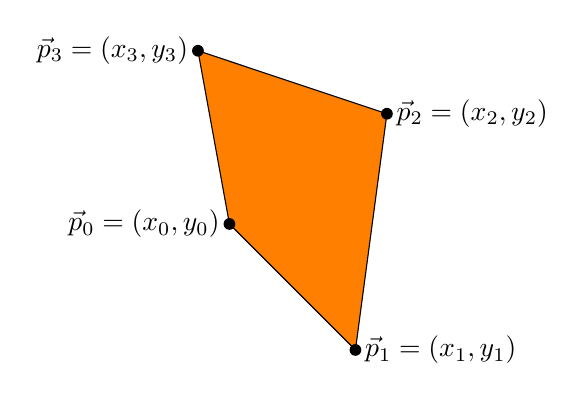
\begin{tikzpicture}[scale=2]
  \coordinate (zero) at (0, 0);
  \coordinate (one) at (0.8, -0.8);
  \coordinate (two) at (1, 0.7);
  \coordinate (three) at (-0.2, 1.1);
  \draw[fill=orange]
    (zero) node[left] {$\vec{p}_0 = (x_0, y_0)$}
    -- (one) node[right] {$\vec{p}_1 = (x_1, y_1)$}
    -- (two) node[right] {$\vec{p}_2 = (x_2, y_2)$}
    -- (three) node[left] {$\vec{p}_3 = (x_3, y_3)$}
    -- cycle;
  \foreach \n in {zero,one,two,three}
    \node at (\n)[circle,fill,inner sep=1.5pt]{};
\end{tikzpicture}

  \textcolor{gray}{\vrule}
  \hspace{0.01\linewidth}
  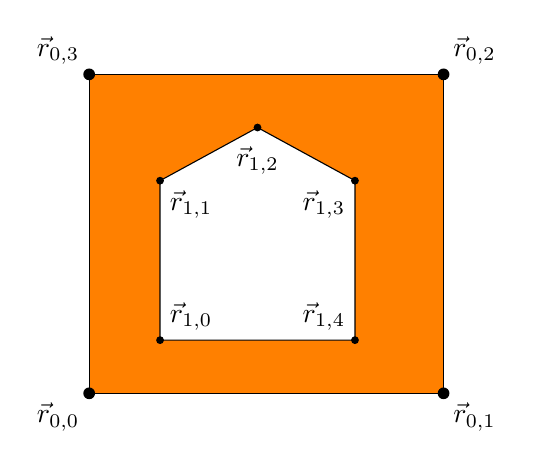
\begin{tikzpicture}[scale=2.25]
  \coordinate (zero) at (0, 0);
  \coordinate (one) at (2.0, 0);
  \coordinate (two) at (2.0, 1.8);
  \coordinate (three) at (0, 1.8);
  \draw[fill=orange]
    (zero) node[below left] {$\vec{r}_{0,0}$}
    -- (one) node[below right] {$\vec{r}_{0,1}$}
    -- (two) node[above right] {$\vec{r}_{0,2}$}
    -- (three) node[above left] {$\vec{r}_{0,3}$}
    -- cycle;
  \foreach \n in {zero,one,two,three}
    \node at (\n)[circle,fill,inner sep=1.5pt]{};

  \coordinate (0) at (0.4, 0.3);
  \coordinate (1) at (1.5, 0.3);
  \coordinate (2) at (1.5, 1.2);
  \coordinate (3) at (0.95, 1.5);
  \coordinate (4) at (0.4, 1.2);
  \draw[fill=white]
    (0) node[above right] {$\vec{r}_{1,0}$}
    -- (1) node[above left] {$\vec{r}_{1,4}$}
    -- (2) node[below left] {$\vec{r}_{1,3}$}
    -- (3) node[below=3.5pt] {$\vec{r}_{1,2}$}
    -- (4) node[below right] {$\vec{r}_{1,1}$}
    -- cycle;
  \foreach \n in {0,1,2,3,4}
    \node at (\n)[circle,fill,inner sep=1pt]{};
\end{tikzpicture}

  \caption{%
    Simple polygon with four unique vertices is shown on the left hand side.
    A complex polygon with an outer hull
    and an interior hull is shown on the right hand side for comparison.
  }%
  \label{fig:polygon-representation}
\end{figure}

A polygon is considered invalid if one or more of its linear rings are self-intersecting, i.e.\ if any of its rings is considered to be complex.
Data providers frequently provide polygons in invalid states and such polygons must be corrected since they are often not processable by common GIS tools.
Zero-buffering invalid polygons (growing the polygon in all directions by zero units) fixes such problems, as can be seen in~\figref{fig:complex-zero-buffer}.

\begin{figure}[H]
  \centering
  \begin{tikzpicture}[scale=1]
  \coordinate (ll) at (0, 0);
  \coordinate (mid) at (2, 1);
  \coordinate (lr) at (4, 0);
  \coordinate (ur) at (4, 2);
  \coordinate (ul) at (0, 2);
  \draw[fill=orange]
    (ll) node[left] {$\vec{r}_0$}
    -- (ur) node[right] {$\vec{r}_1$}
    -- (lr) node[right] {$\vec{r}_2$}
    -- (ul) node[left] {$\vec{r}_3$}
    -- cycle;
  \foreach \n in {ll,ur,lr,ul}
    \node at (\n)[circle,fill,inner sep=1.5pt]{};

   \draw (4.4, 1) edge[->, thick] node[above] {\texttt{buffer(0.0)}} (6.6, 1);

  \coordinate (offset) at (7, 0);
  \draw[fill=orange]
    ($ (ll) + (offset) $) node[left] {$\vec{r}_0$}
    -- ($ (mid) + (offset) $) node[below] {$\vec{r}_1$}
    -- ($ (lr) + (offset) $) node[right] {$\vec{r}_2$}
    -- ($ (ur) + (offset) $) node[right] {$\vec{r}_3$}
    -- ($ (mid) + (offset) $) node[above] {$\vec{r}_4$}
    -- ($ (ul) + (offset) $) node[left] {$\vec{r}_5$}
    -- cycle;
  \foreach \n in {ll,mid,lr,ur,mid,ul}
    \node at ($ (\n) + (offset) $)[circle,fill,inner sep=1.5pt]{};
\end{tikzpicture}

  \caption{Illustration of how zero-buffering an invalid polygon corrects self-intersecting polygons.}%
  \label{fig:complex-zero-buffer}
\end{figure}

Zero-buffering polygons has the added benefit of normalizing vector data by re-ordering the polygon vertices in an anti-clockwise manner and removing redundant vertices as shown in~\figref{fig:redundant-zero-buffer}.

\begin{figure}[H]
  \centering
  \begin{tikzpicture}[scale=1]
  \coordinate (ll) at (0, 0);
  \coordinate (lm) at (2, 0);
  \coordinate (lr) at (4, 0);
  \coordinate (ur) at (4, 1);
  \coordinate (um) at (2, 1);
  \coordinate (Um) at (2, 2);
  \coordinate (ul) at (0, 1);
  \draw[fill=orange]
    (ll) node[below] {$\vec{r}_0$}
    -- (lm) node[below] {$\vec{r}_1$}
    -- (lr) node[below] {$\vec{r}_2$}
    -- (ur) node[above] {$\vec{r}_3$}
    -- (um) node[above right] {$\vec{r}_4$}
    -- (Um) node[above] {$\vec{r}_5$}
    -- (um) node[above left] {$\vec{r}_6$}
    -- (ul) node[above] {$\vec{r}_7$}
    -- cycle;
  \foreach \n in {ll,lm,lr,ur,um,Um,um,ul}
    \node at (\n)[circle,fill,inner sep=1.5pt]{};

   \draw (4.9, 0.5) edge[->, thick] node[above] {\texttt{buffer(0.0)}} (7.1, 0.5);

  \coordinate (offset) at (8, 0);
  \draw[fill=orange]
    ($ (ll) + (offset) $) node[below] {$\vec{r}_0$}
    -- ($ (lr) + (offset) $) node[below] {$\vec{r}_1$}
    -- ($ (ur) + (offset) $) node[above] {$\vec{r}_2$}
    -- ($ (ul) + (offset) $) node[above] {$\vec{r}_3$}
    -- cycle;
  \foreach \n in {ll,lr,ur,ul}
    \node at ($ (\n) + (offset) $)[circle,fill,inner sep=1.5pt]{};
\end{tikzpicture}

  \caption{Illustration of how zero-buffering polygons removes redundant vertices.}%
  \label{fig:redundant-zero-buffer}.
\end{figure}

This allows you to apply simpler similarity measures for comparing polygons, and reduces computational costs when processing the polygons.
Technical details for applying zero-buffers to vector data is provided in~\appref{app:zero-buffer}.
We will come back to how to combine vector and raster datasets by \textit{rasterization} in~\secref{sec:masking} where it will also become clear why the removal of redundant vertices is of importance.


\subsubsection{Raster data}
Raster data is simply scalar measurements imposed onto a grid with rectangular grid cells.

A color image, $I$, of width $\mathrm{W}$ and height $\mathrm{H}$, for instance, will contain three color channels,
\textcolor{red}{red}, \textcolor{green}{green}, and \textcolor{blue}{blue}, (RGB)
and can be represented by a three-dimensional array of size $\mathrm{W} \times \mathrm{H} \times \mathrm{3}$.
Each color channel in a given pixel is represented by an unsigned 8-bit integer, i.e.
\begin{equation*}
  I_{i, j, c} \in \{0, 1, \ldots, 255\},
  \hspace{2.5em}
  i = 0, \ldots, \mathrm{H} - 1,
  ~~
  j = 0, \ldots, \mathrm{W} - 1,
  ~~
  c = \mathrm{\textcolor{red}{R}, \textcolor{green}{G},\textcolor{blue}{B}}.
\end{equation*}

A LiDAR height map, $Z$, is likewise encoded as a single-channel grayscale image of size $\mathrm{W} \times \mathrm{H}$.
Each pixel is represented by a signed 32-bit floating point value, i.e.
\begin{equation*}
  Z_{i, j} \in \mathbb{R},
  \hspace{2.5em}
  i = 0, \ldots, \mathrm{H} - 1,
  ~~
  j = 0, \ldots, \mathrm{W} - 1.
\end{equation*}

These two raster types must be handled differently during data normalization due to their different value domains, which we will come back to in~\secref{sec:raster-normalization}.

% Do not split the following section over different pages
\begin{minipage}{\textwidth}
  For GIS rasters we must define the spatial extent of the given image as well, specified by:
  \begin{itemize}[noitemsep]
    \item A coordinate system, for example UTM \texttt{32V}.
    \item The coordinate of the center of the upper left pixel, $I_{1, 1}$; the \textit{origin} $\vec{r}_0 = {[x_0, y_0]}^T$.
    \item The pixel step size, $\vec{\Delta} = {[\Delta_x, \Delta_y]}^T$, for example ${[\SI{0.25}{\meter}, \SI{-0.25}{\meter}]}^T$.
  \end{itemize}
\end{minipage}
\vspace{0.5em}

The pixel $I_{i, j, c}$ therefore represents a rectangle of width $\Delta_x$ and height $\Delta_y$ centered at the spatial coordinate $\vec{r}_0 + \vec{\Delta} \cdot [i, j]$, everything being interpreted in the given coordinate system.

Missing data in remote sensing rasters are specified by filling in a pre-defined \texttt{nodata} placeholder value.
For RGB data this is often set to $0$, resulting in a black pixel.
LiDAR rasters often use $\texttt{nodata} = -2^{127} \times (2 - 2^{-23}) \approx 3.4028234664 \times 10^{38}$, the smallest normal number representable by a single-precision floating point number.
Such \texttt{nodata} values may arise from measurement errors and regions which are outside the given covarage area of the dataset, and must be special-cased during data normalization, which we will come back to in~\secref{sec:raster-normalization}.

\subsubsection*{Merging raster datasets}

Aerial photography and LiDAR data is usually provided in several smaller raster files, organized in a tiled pattern in order to reduce file sizes.
Each file is a \texttt{.geotiff} file, a container format which specifies necessary metadata and the underlying image data in a lossless format such as \texttt{PNG}.
This poses the problem of having to look up which files that cover a given region of interest and merging these files together before processing them.

A simpler approach is to create a \textit{GDAL Virtual Format} file (\texttt{VRT}) which is a virtual dataset file referencing all the respective tiles and bands (GIS uses the term bands for what we would otherwise refer to as image channels).
In simple cases, a \texttt{VRT} file can be autogenerated with the \texttt{gdalbuildvrt} GDAL utility.

\begin{shellcode}
$ gdalbuildvrt raster.vrt ${raster_directory}/*.tif
\end{shellcode}
%
The resulting \texttt{vrt} file behaves like single merged file, and can be read and processed by most GIS tools, but in practice it is just a small XML file and does not require you to load the entire raster dataset into memory.

Using the same file format, we can also combine overlapping raster datasets by expanding the number of channels in the resulting raster.

\begin{shellcode}
$ gdalbuildvrt -resolution ${resolution} combined.vrt -separate ${vrt1} ${vrt2} 
\end{shellcode}
%
Where \texttt{-resolution} can be set to either \texttt{highest}, \texttt{lowest}, or \texttt{average}, depending on how you want to handle datasets with different resolutions.
This is how we will merge the aerial photography (RGB) data with the DSM data (Z), resulting in a single consistent ZRGB dataset.
The resulting \texttt{VRT} file will only contain the first band from each source file, and needs to be manually edited according to the VRT schema~\cite{vrt_schema_2015} in order to include the green and blue bands of the original RGB dataset.


\subsection{Data sets}

\subsubsection{LiDAR data}
\todo{Write about LiDAR data.}


\subsubsection{Building data}
\todo{
  Write about Trondheim building data set, provided in \\
  \texttt{Basisdata\_5001\_Trondheim\_5972\_FKB-Bygning\_GML.gml}.
}


\subsubsection{Summary of data sets}
\begin{table}[htb]
  \centering
  \resizebox{\textwidth}{!}{%
    \begin{tabular}{lSSrrrr}
      \toprule
      {Data set} & {Resolution} & {Size} & {Coverage area} & {Date} & Scan angle & Accuracy \\
      \midrule
      Orthophoto~\cite{trondheim_ortophoto_2017} & \SIrange{0.04}{0.15}{\meter} & \SI{161}{\giga\byte}  & TODO & \date{2017} & {} & \SI{\pm 0.35}{\meter} \\
      LiDAR~\cite{trondheim_lidar_2017} & \SI{0.2}{\meter} & \SI{25}{\giga\byte} & \SI{342}{\kilo\meter\squared} & \date{2017-10-10} & \SI{\pm 20}{\degree} & \SI{\pm 0.02}{\meter} (SD) \\
      \bottomrule
    \end{tabular}%
  }
\end{table}

\begin{table}[htb]
  \centering
  \begin{tabular}{cc}
    \toprule
    {Point density (\si{\per\meter\squared})} & {Proportion (\%)} \\
    \midrule
    $> 100\%$ & 97.7 \\
    \SIrange{85}{100}{\percent} & 1.2 \\
    \SIrange{60}{85}{\percent} & 1.1 \\
    \bottomrule
  \end{tabular}
  \caption{
    Control of point cloud density of the Trondheim 2017 LiDAR data set.
    The densities are calculated within rolling windows of size $\SI{10}{\meter} \times \SI{10}{\meter}$~\cite{trondheim_lidar_2017}.
    }
\end{table}

Pixel domain is $(1, 254)$ for all three color channels.
\SI{70.77}{\percent} of all pixels are valid, probably due to lower resolution than the actual resolution.
Elevation data is in domain $(-9.390, 569.050)$.

